\section*{Tenant}

\subsection*{Create new tenant}

\begin{itemize}
  \item[] \textbf{Trigger:} User interaction with CMS window
  \item[] \textbf{Precondition:} Assert that user has logged in
  \item[] \textbf{Path:}
    \begin{enumerate}
      \item User clicks Admin on navigation bar
      \item User clicks on Tenants in the dropdown
      \item User clicks ``New Tenant'' button
      \item User fills the tenant information in the form
      \item User clicks ``Create Tenant'' button
      \item ``Tenant successfully created'' message is shown together with the data
    \end{enumerate}
  \item[] \textbf{Requirements:}
    \begin{enumerate}
      \item The new tenant's data should be added to the database
      \item The new tenant's information should be displayed in the homepage correctly
      \item The tenants' information should be listed in the creation order
    \end{enumerate}
  \item[] \textbf{Screenshots:} \\
    \includegraphics[scale=0.25]{./images/ss/tenant/create/1.png}
    \includegraphics[scale=0.25]{./images/ss/tenant/create/2.png}\\
    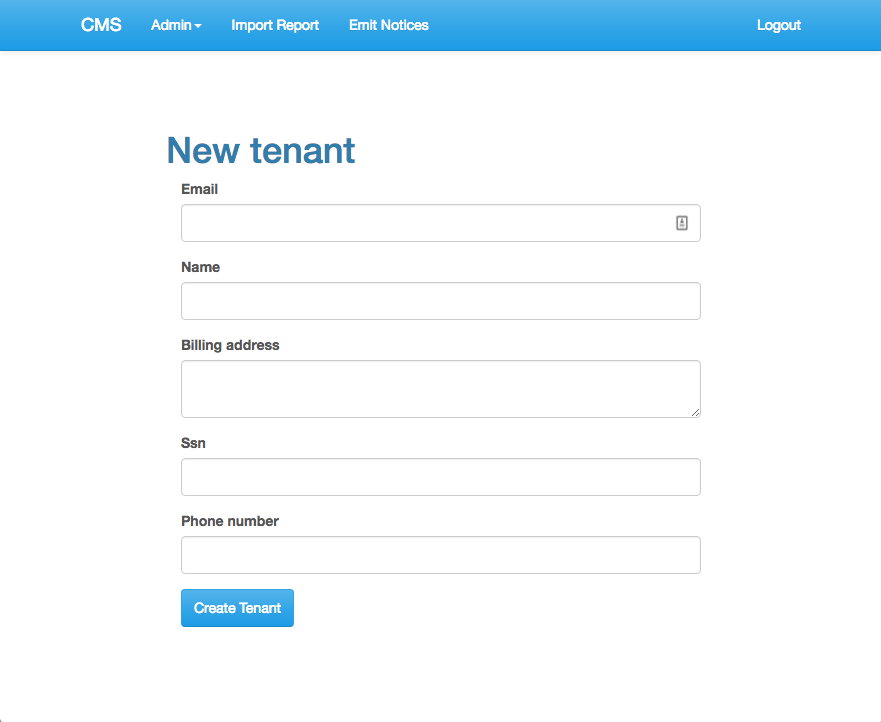
\includegraphics[scale=0.25]{./images/ss/tenant/create/3.png}
    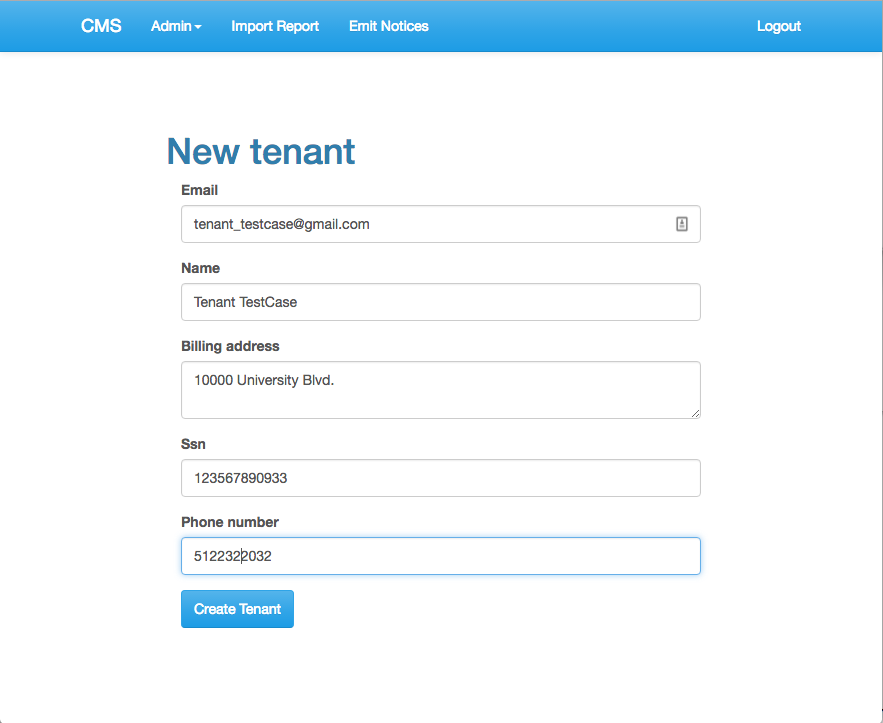
\includegraphics[scale=0.25]{./images/ss/tenant/create/4.png}\\
    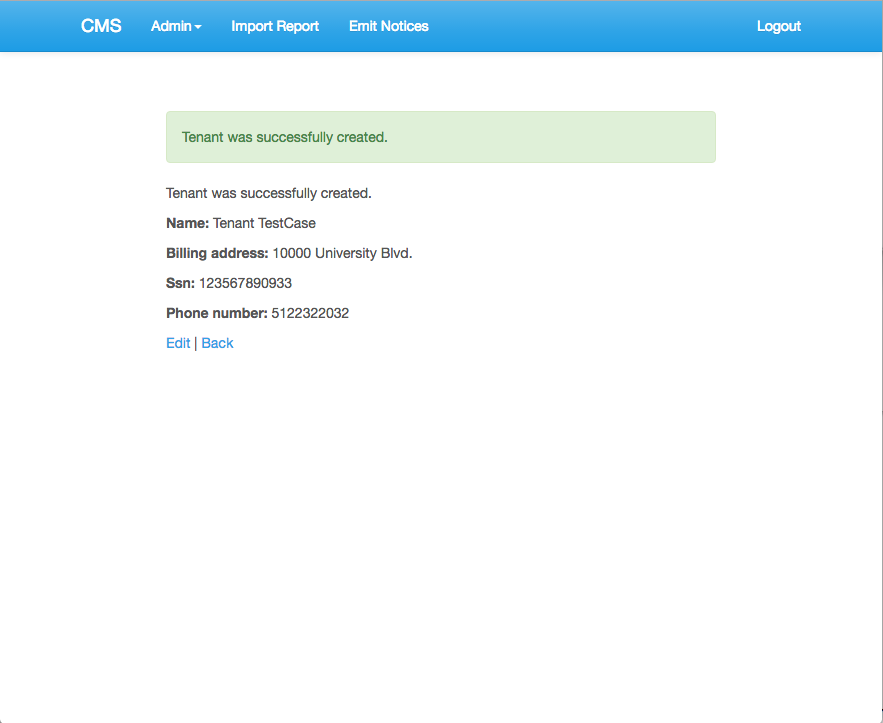
\includegraphics[scale=0.25]{./images/ss/tenant/create/5.png}
\end{itemize}

\subsection*{Edit a tenant}

\begin{itemize}
  \item[] \textbf{Trigger:} User interaction with CMS window
  \item[] \textbf{Precondition:} Assert that user is in the Tenant page and the tenant to edit is existed
  \item[] \textbf{Path:}
    \begin{enumerate}
      \item User clicks on Edit behind the information of the tenant who will be edited
      \item User edit new information in the form
      \item User clicks ``Update Tenant'' button
      \item ``Tenant successfully updated'' massage is shown
    \end{enumerate}
  \item[] \textbf{Requirements:}
    \begin{enumerate}
      \item The updated tenant’s new data should be updated to the database
      \item The updated tenant’s new information should be displayed in the homepage correctly
      \item The tenants’ information should be listed in the modification order
    \end{enumerate}
  \item[] \textbf{Screenshots:}\\
    \includegraphics[scale=0.25]{./images/ss/tenant/edit/1.png}
    \includegraphics[scale=0.25]{./images/ss/tenant/edit/2.png}\\
    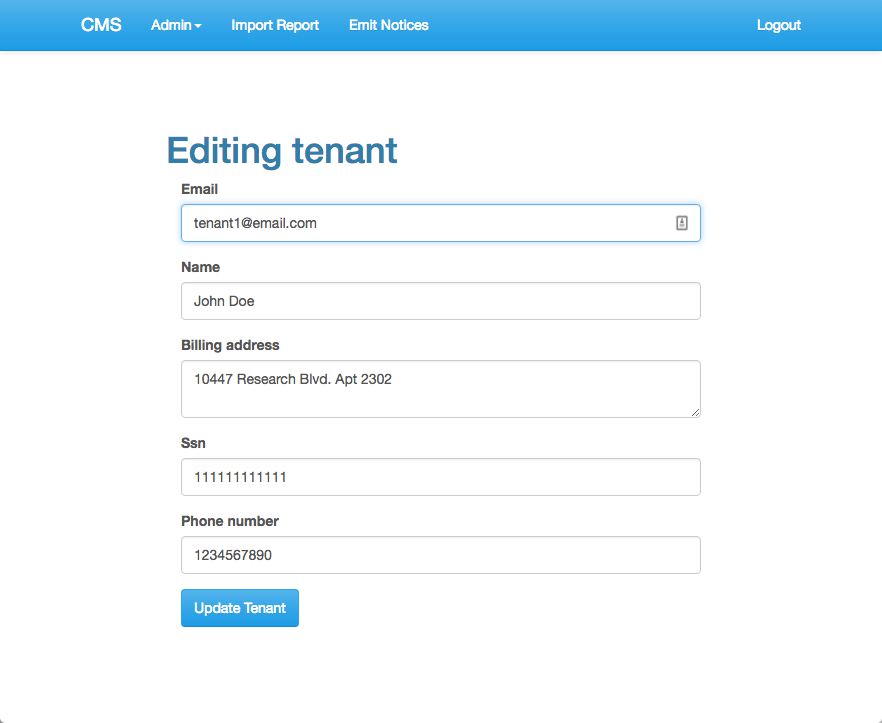
\includegraphics[scale=0.25]{./images/ss/tenant/edit/3.png}
    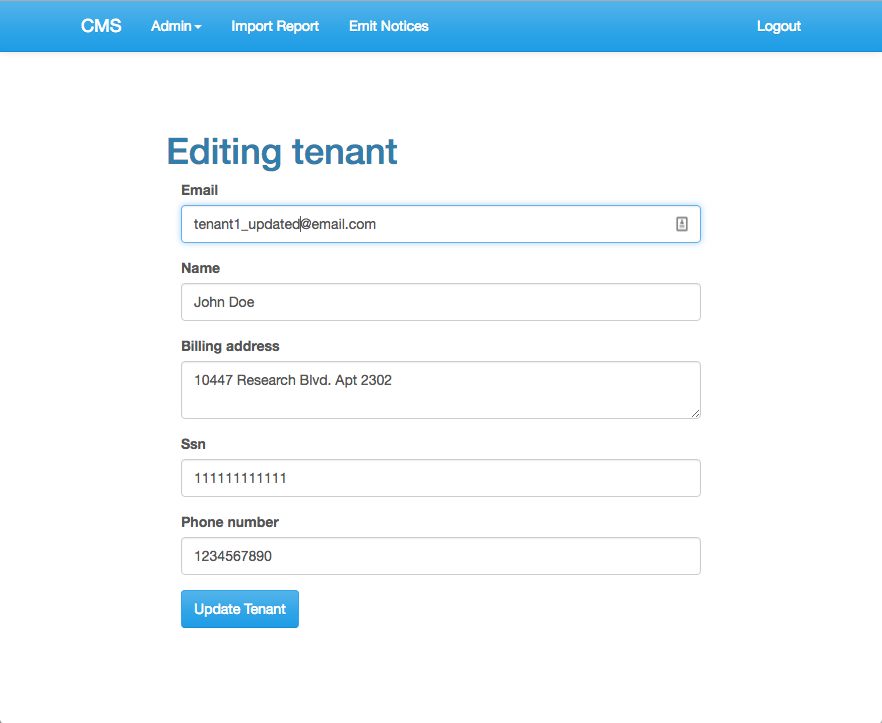
\includegraphics[scale=0.25]{./images/ss/tenant/edit/4.png}\\
    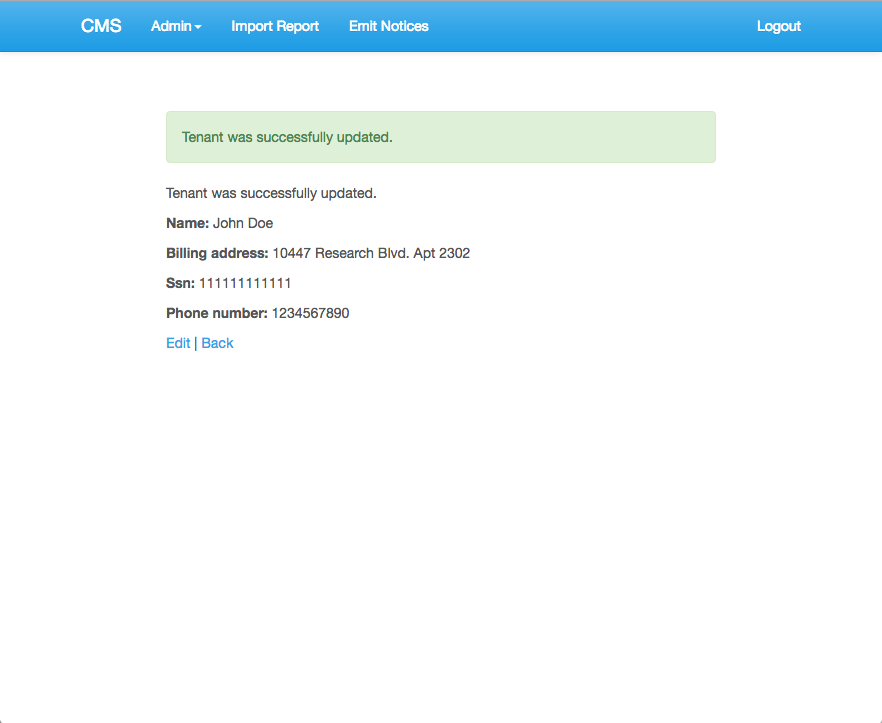
\includegraphics[scale=0.25]{./images/ss/tenant/edit/5.png}
\end{itemize}

\subsection*{Delete a tenant}

\begin{itemize}
  \item[] \textbf{Trigger:} User interaction with CMS window
  \item[] \textbf{Precondition:} Assert that user is in the Tenant page and the tenant to edit is existed
  \item[] \textbf{Path:}
    \begin{enumerate}
      \item User clicks on Destroy at the end of the information of the tenant who will be deleted
      \item An alter message says ``Are you sure'' is shown
      \item User clicks ``OK'' button
      \item Tenant successfully destroyed massage is shown
    \end{enumerate}
  \item[] \textbf{Requirements:}
    \begin{enumerate}
      \item The deleted tenant’s data should be removed to the database
      \item The deleted tenant’s information should not be displayed in the homepage
      \item Other tenants’ information should be listed as the same as those before deleting
    \end{enumerate}
  \item[] \textbf{Screenshots:}\\
    \includegraphics[scale=0.25]{./images/ss/tenant/delete/1.png}
    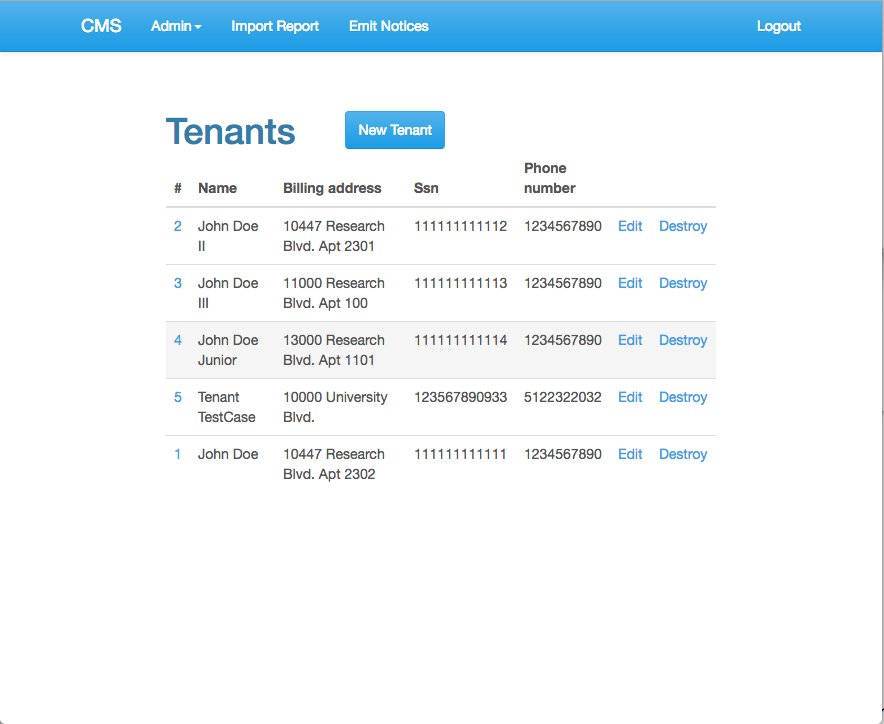
\includegraphics[scale=0.25]{./images/ss/tenant/delete/2.png}\\
    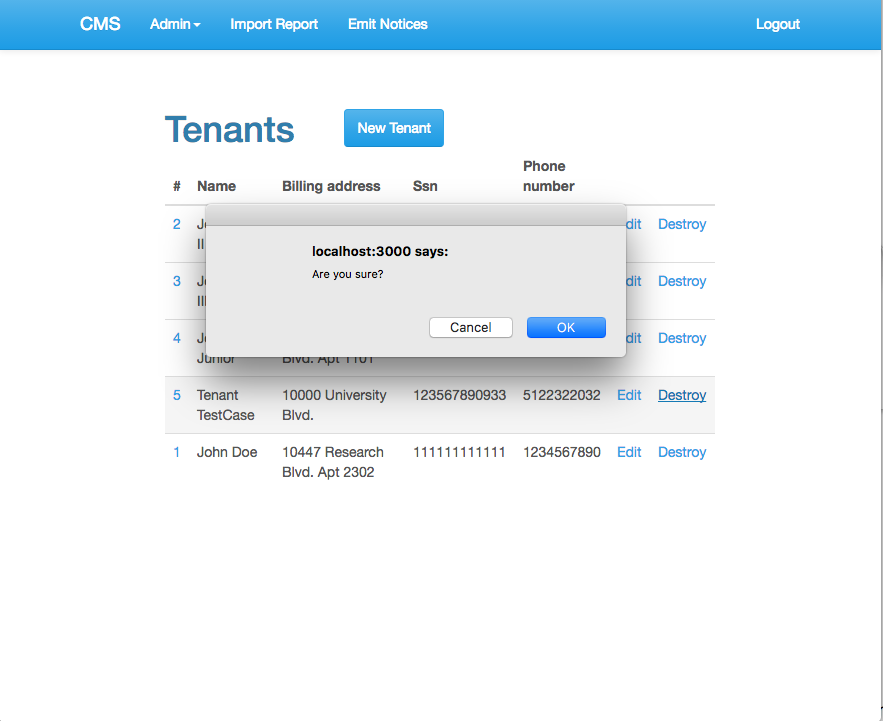
\includegraphics[scale=0.25]{./images/ss/tenant/delete/3.png}
    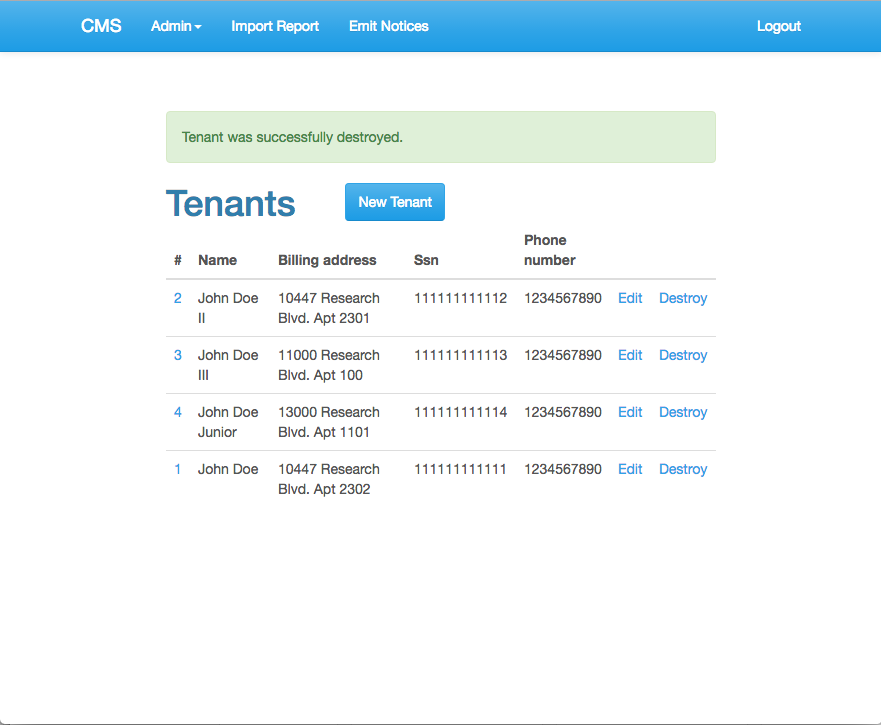
\includegraphics[scale=0.25]{./images/ss/tenant/delete/4.png}
\end{itemize}
